\documentclass{article}

\usepackage{amsmath}
\usepackage{amsthm}

%%%%%%%%%%%%%%%%%%%%%%%%%%%%%%%%%%%%%%%%
                                       %
% change this line for portable code:  %
\newcommand*{\commonDir}{./common/}    %
\input{\commonDir preambleCommon}      %
                                       %
%%%%%%%%%%%%%%%%%%%%%%%%%%%%%%%%%%%%%%%%

\graphicspath{{./epistasisEnvFBA/figures/}}

\begin{document}

\begin{figure}[H]
\caption{}
\label{fig:eef1}
\centering
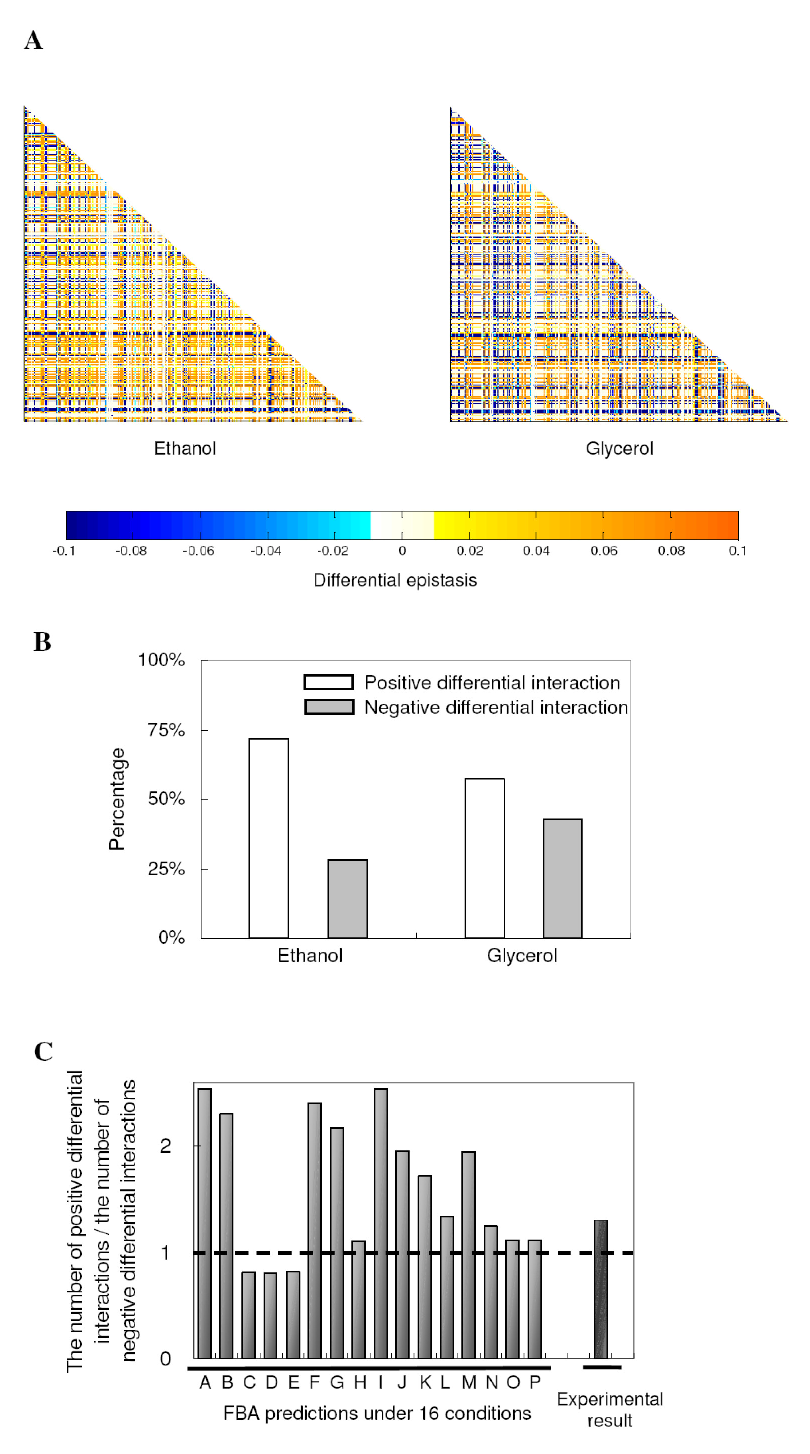
\includegraphics[height=0.95\textheight]{envFigure_1}
\end{figure}

\begin{figure}[H]
\caption{}
\label{fig:eef2}
\centering
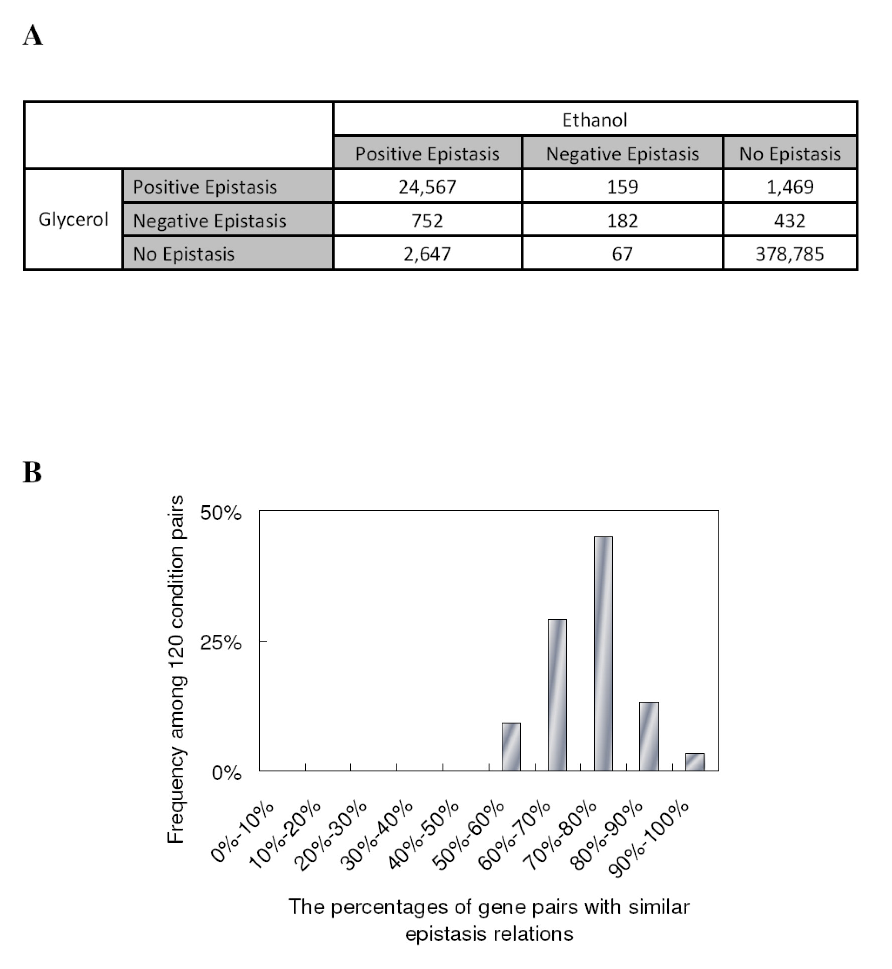
\includegraphics[width=\textwidth]{envFigure_2}
\end{figure}

\begin{figure}[H]
\caption{}
\label{fig:eef3}
\centering
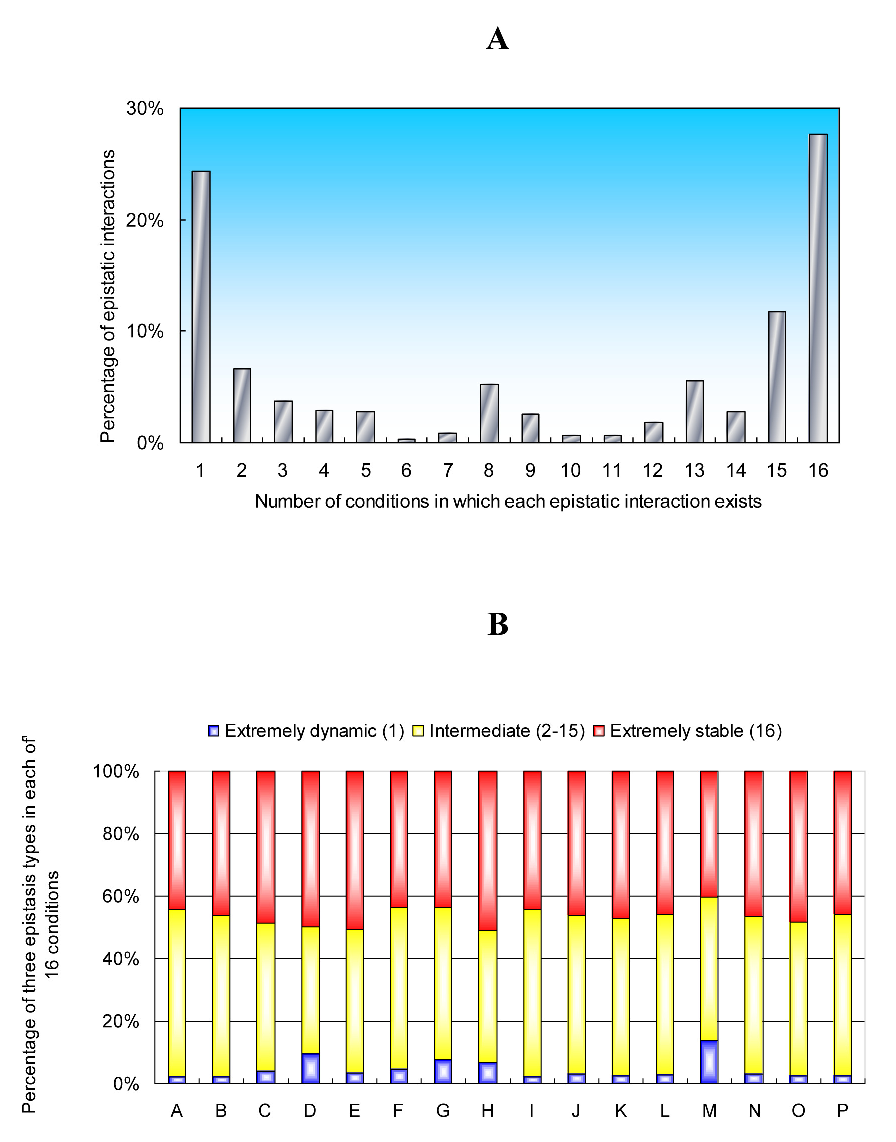
\includegraphics[width=\textwidth]{envFigure_3}
\end{figure}

\begin{figure}[H]
\caption{}
\label{fig:eef4}
\centering
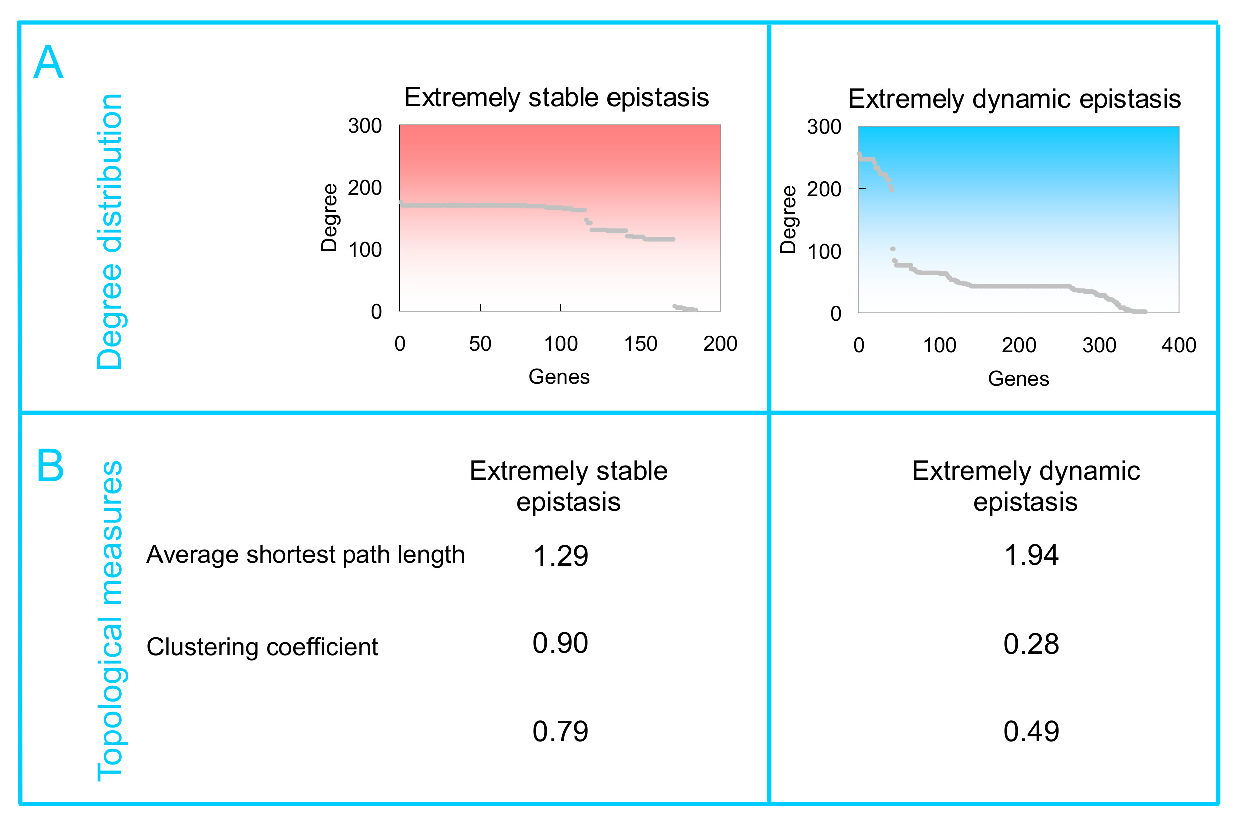
\includegraphics[width=\textwidth]{envFigure_4}
\end{figure}

\begin{figure}[H]
\caption{}
\label{fig:eef5}
\centering
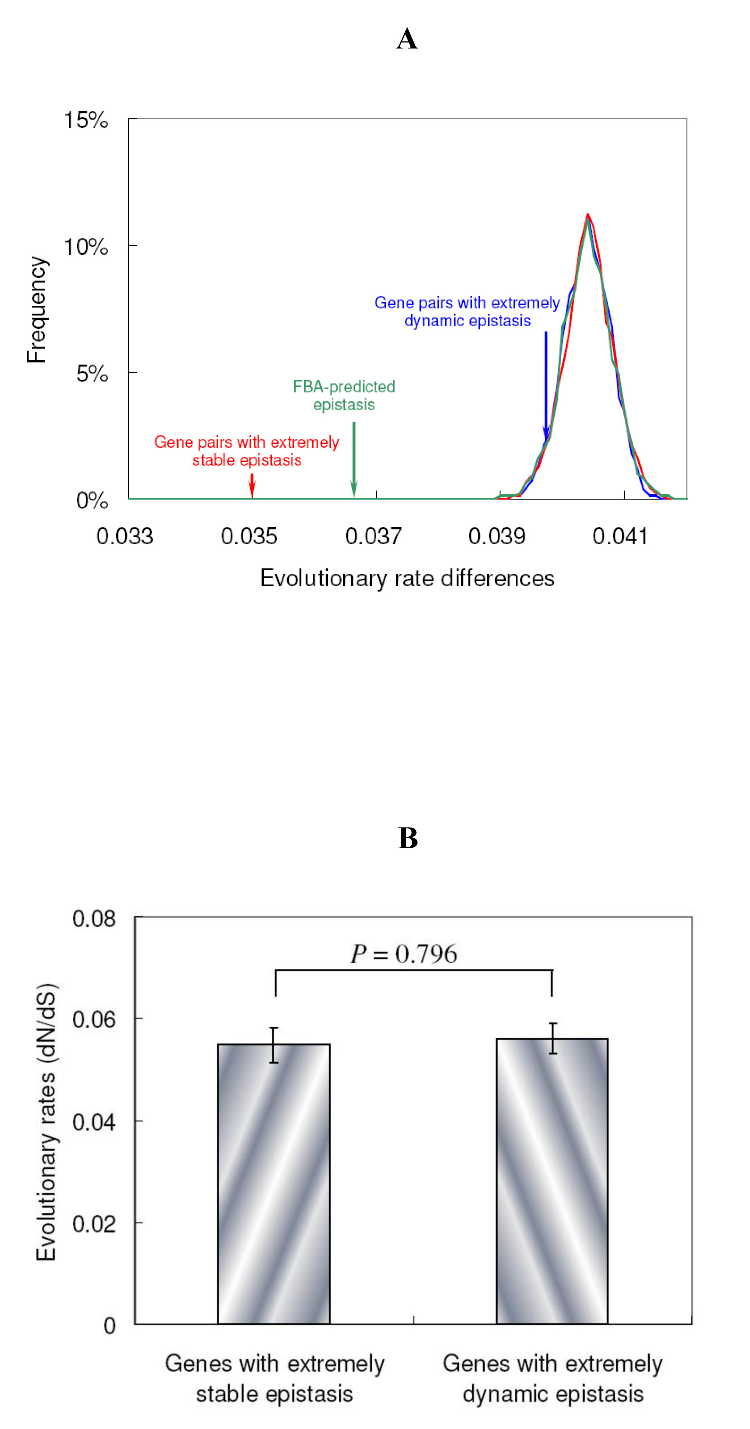
\includegraphics[height=0.95\textheight]{envFigure_5}
\end{figure}


%%%%%%%%%%%%%%%%%%%%%%%%%%%%%%%%%%%%%%%%%%%%%%%%%%
                                                 %
\setcounter{figure}{0}                           %
\makeatletter                                    %
\renewcommand{\thefigure}{S\@arabic\c@figure}    %
\makeatother                                     %
                                                 %
%%%%%%%%%%%%%%%%%%%%%%%%%%%%%%%%%%%%%%%%%%%%%%%%%%

\begin{figure}[H]
\caption{}
\label{fig:eefS1}
\centering
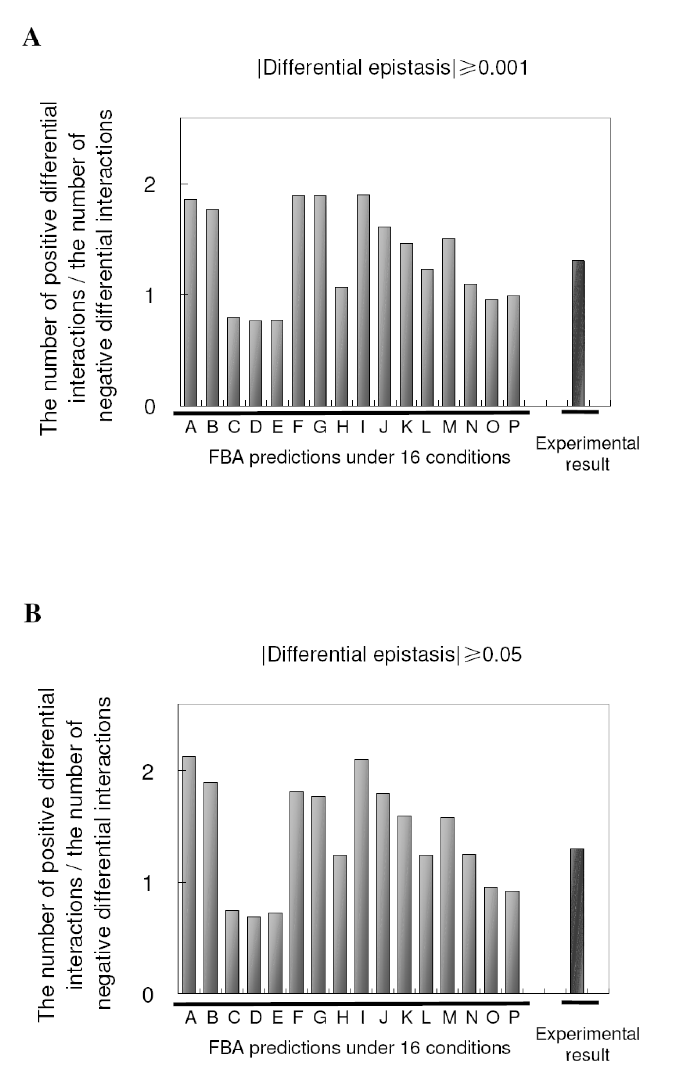
\includegraphics[height=0.97\textheight]{envFigure_S1}
\end{figure}

\begin{figure}[H]
\caption{}
\label{fig:eefS2}
\centering
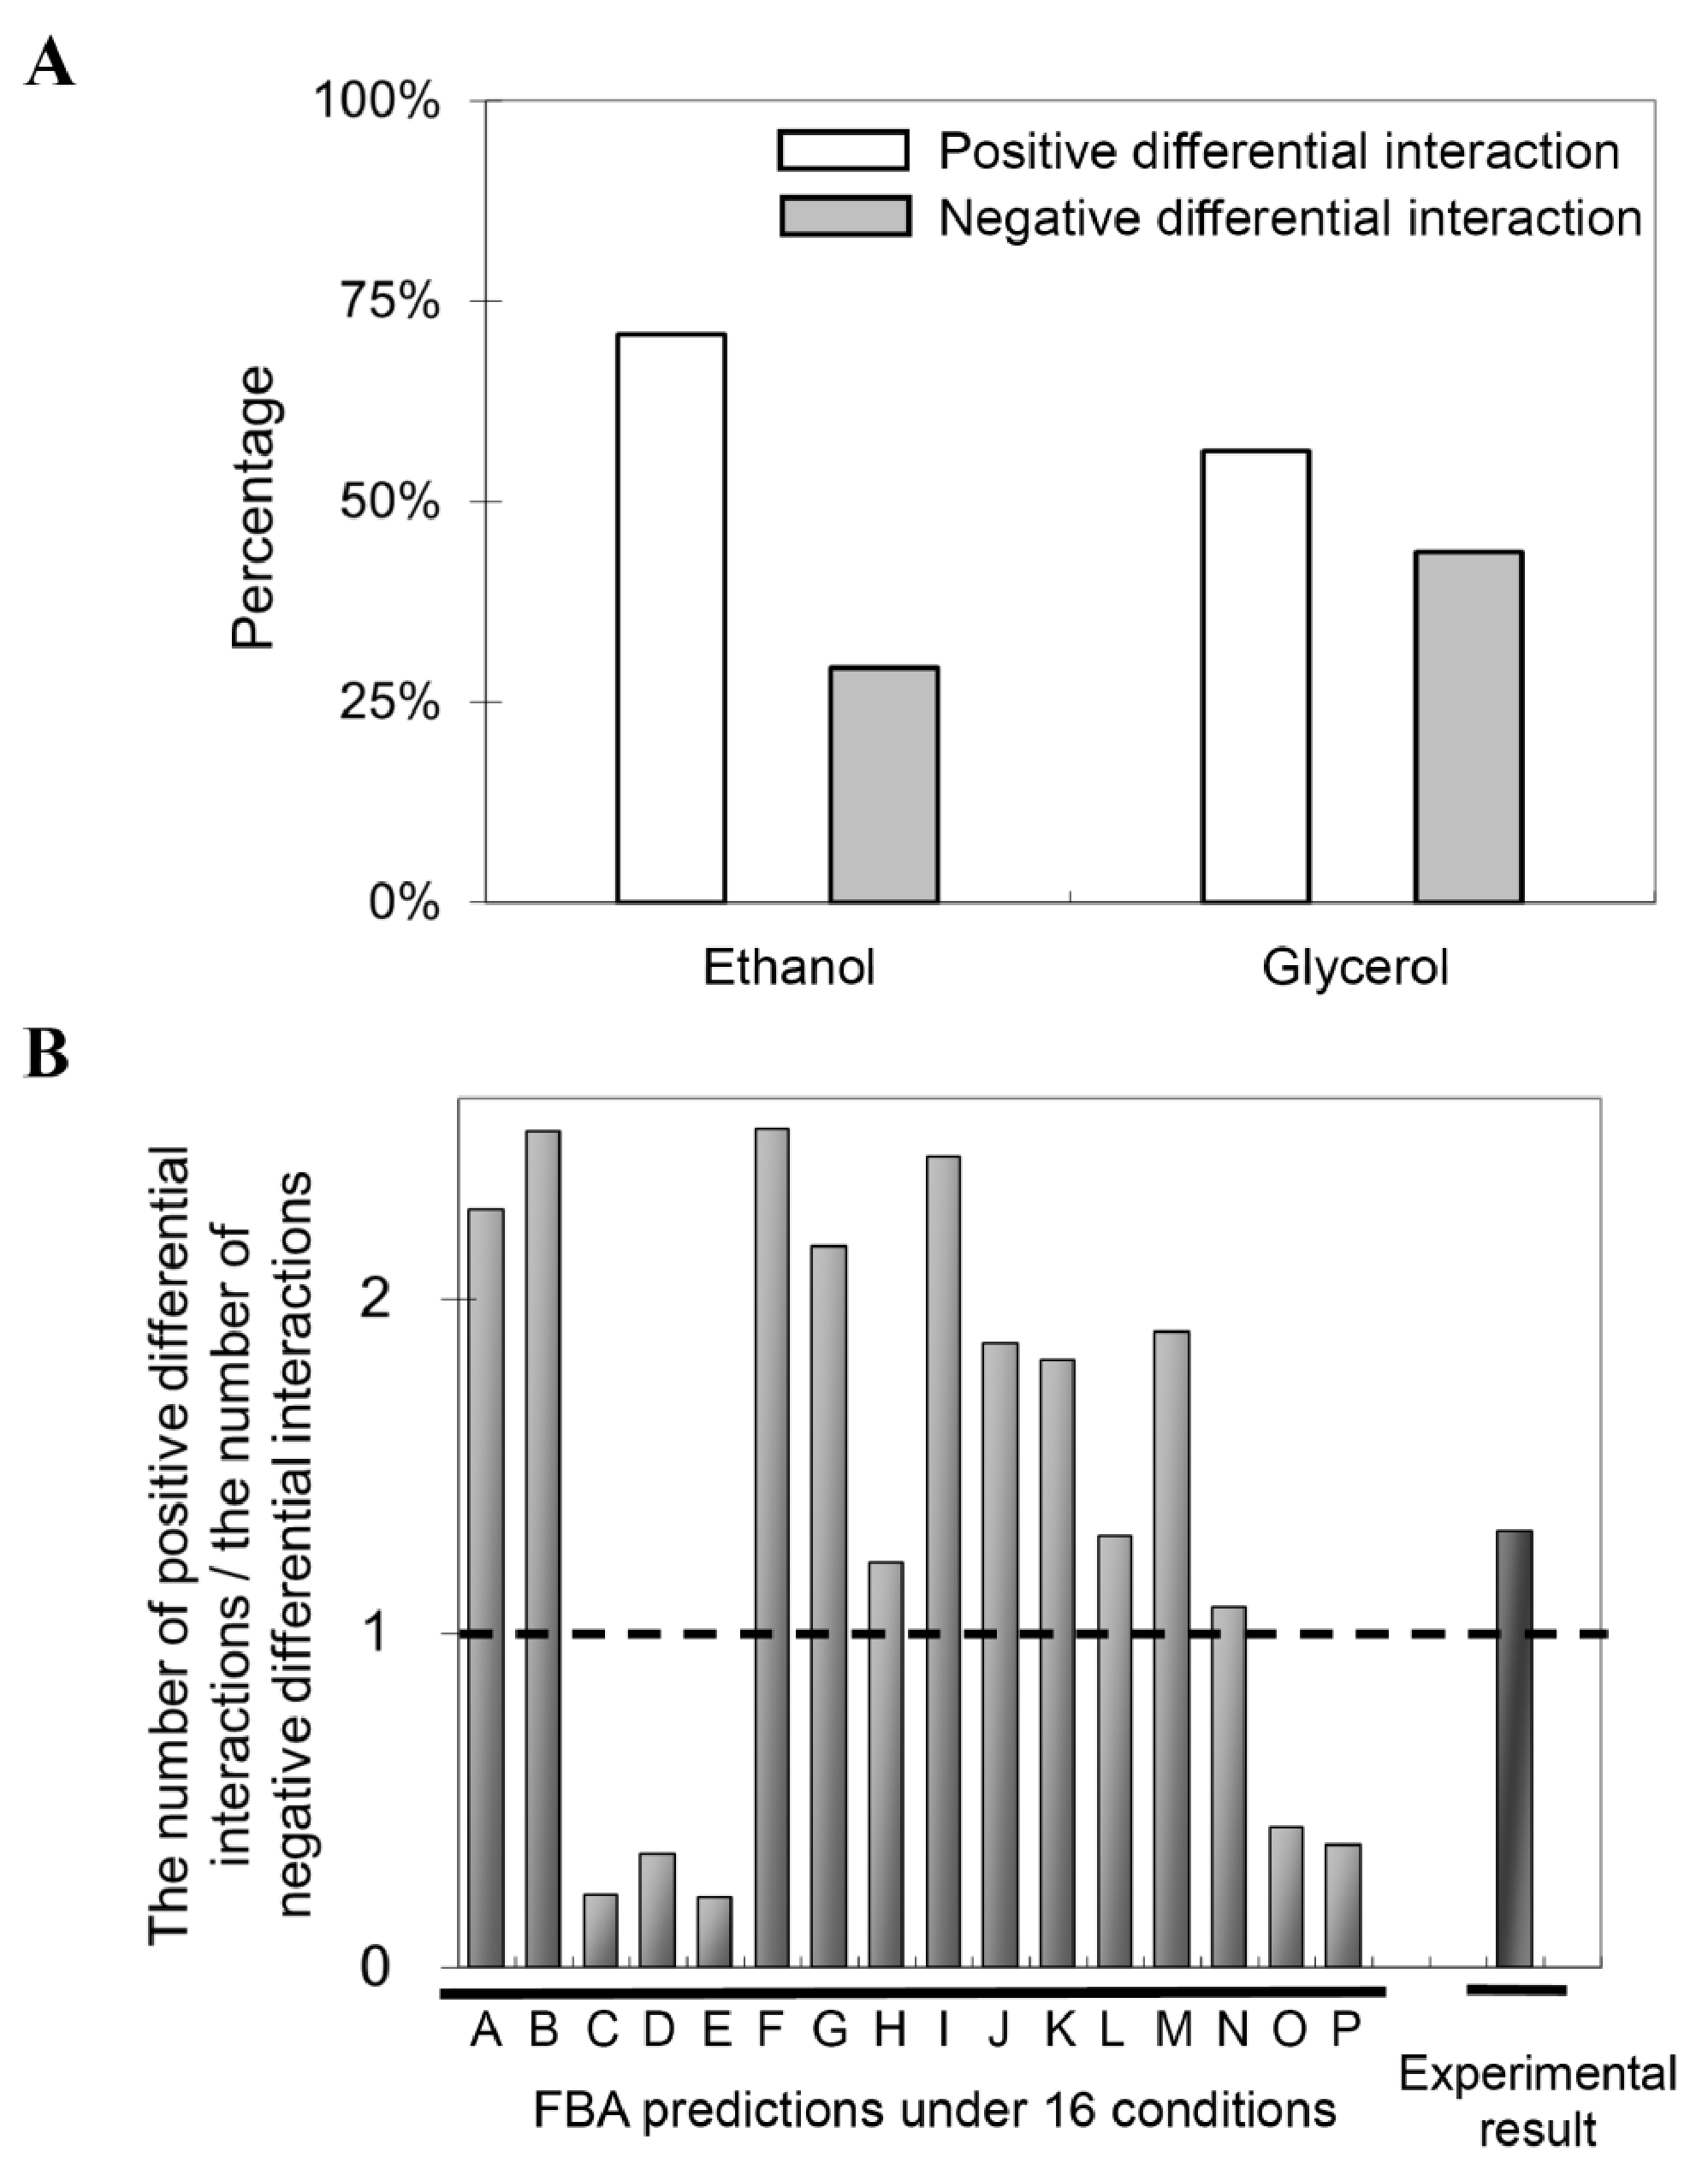
\includegraphics[width=\textwidth]{envFigure_S2}
\end{figure}

\begin{figure}[H]
\caption{}
\label{fig:eefS3}
\centering
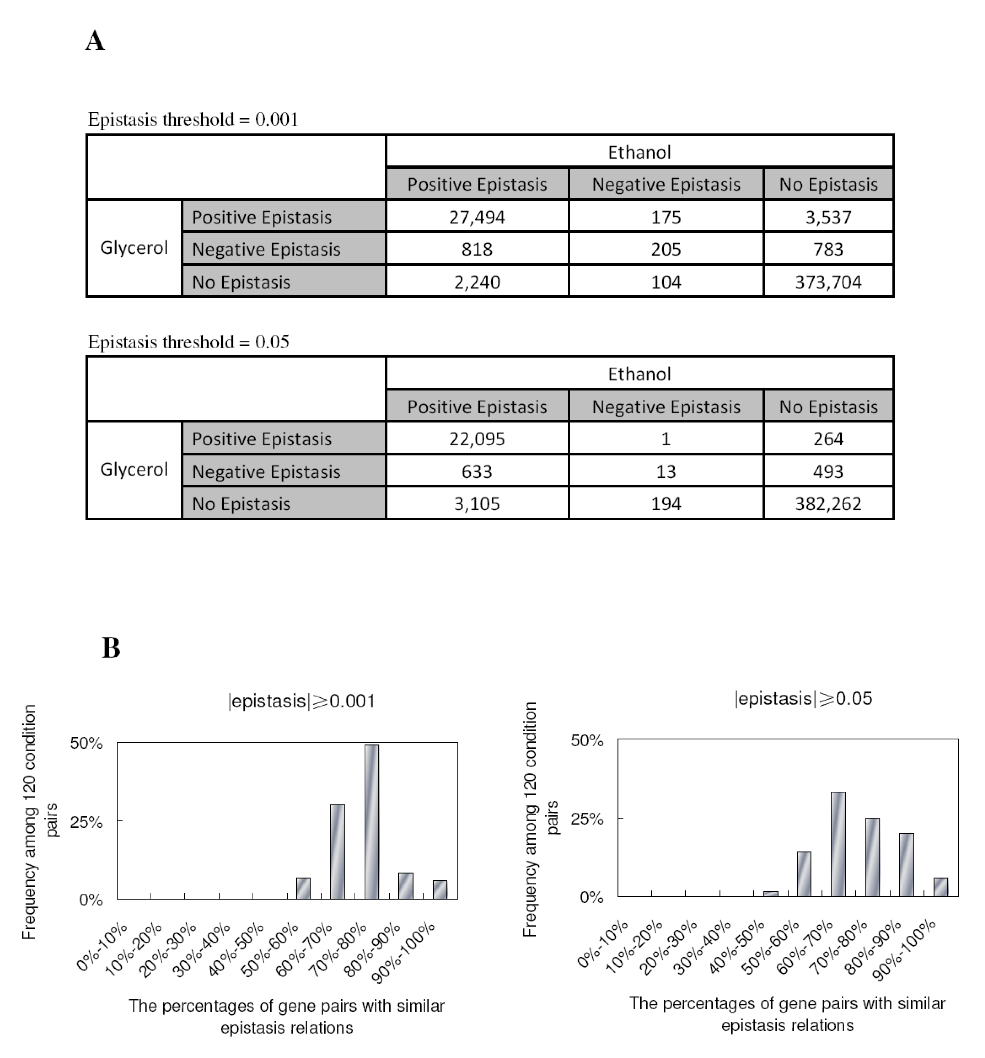
\includegraphics[width=\textwidth]{envFigure_S3}
\end{figure}

\begin{figure}[H]
\caption{}
\label{fig:eefS4}
\centering
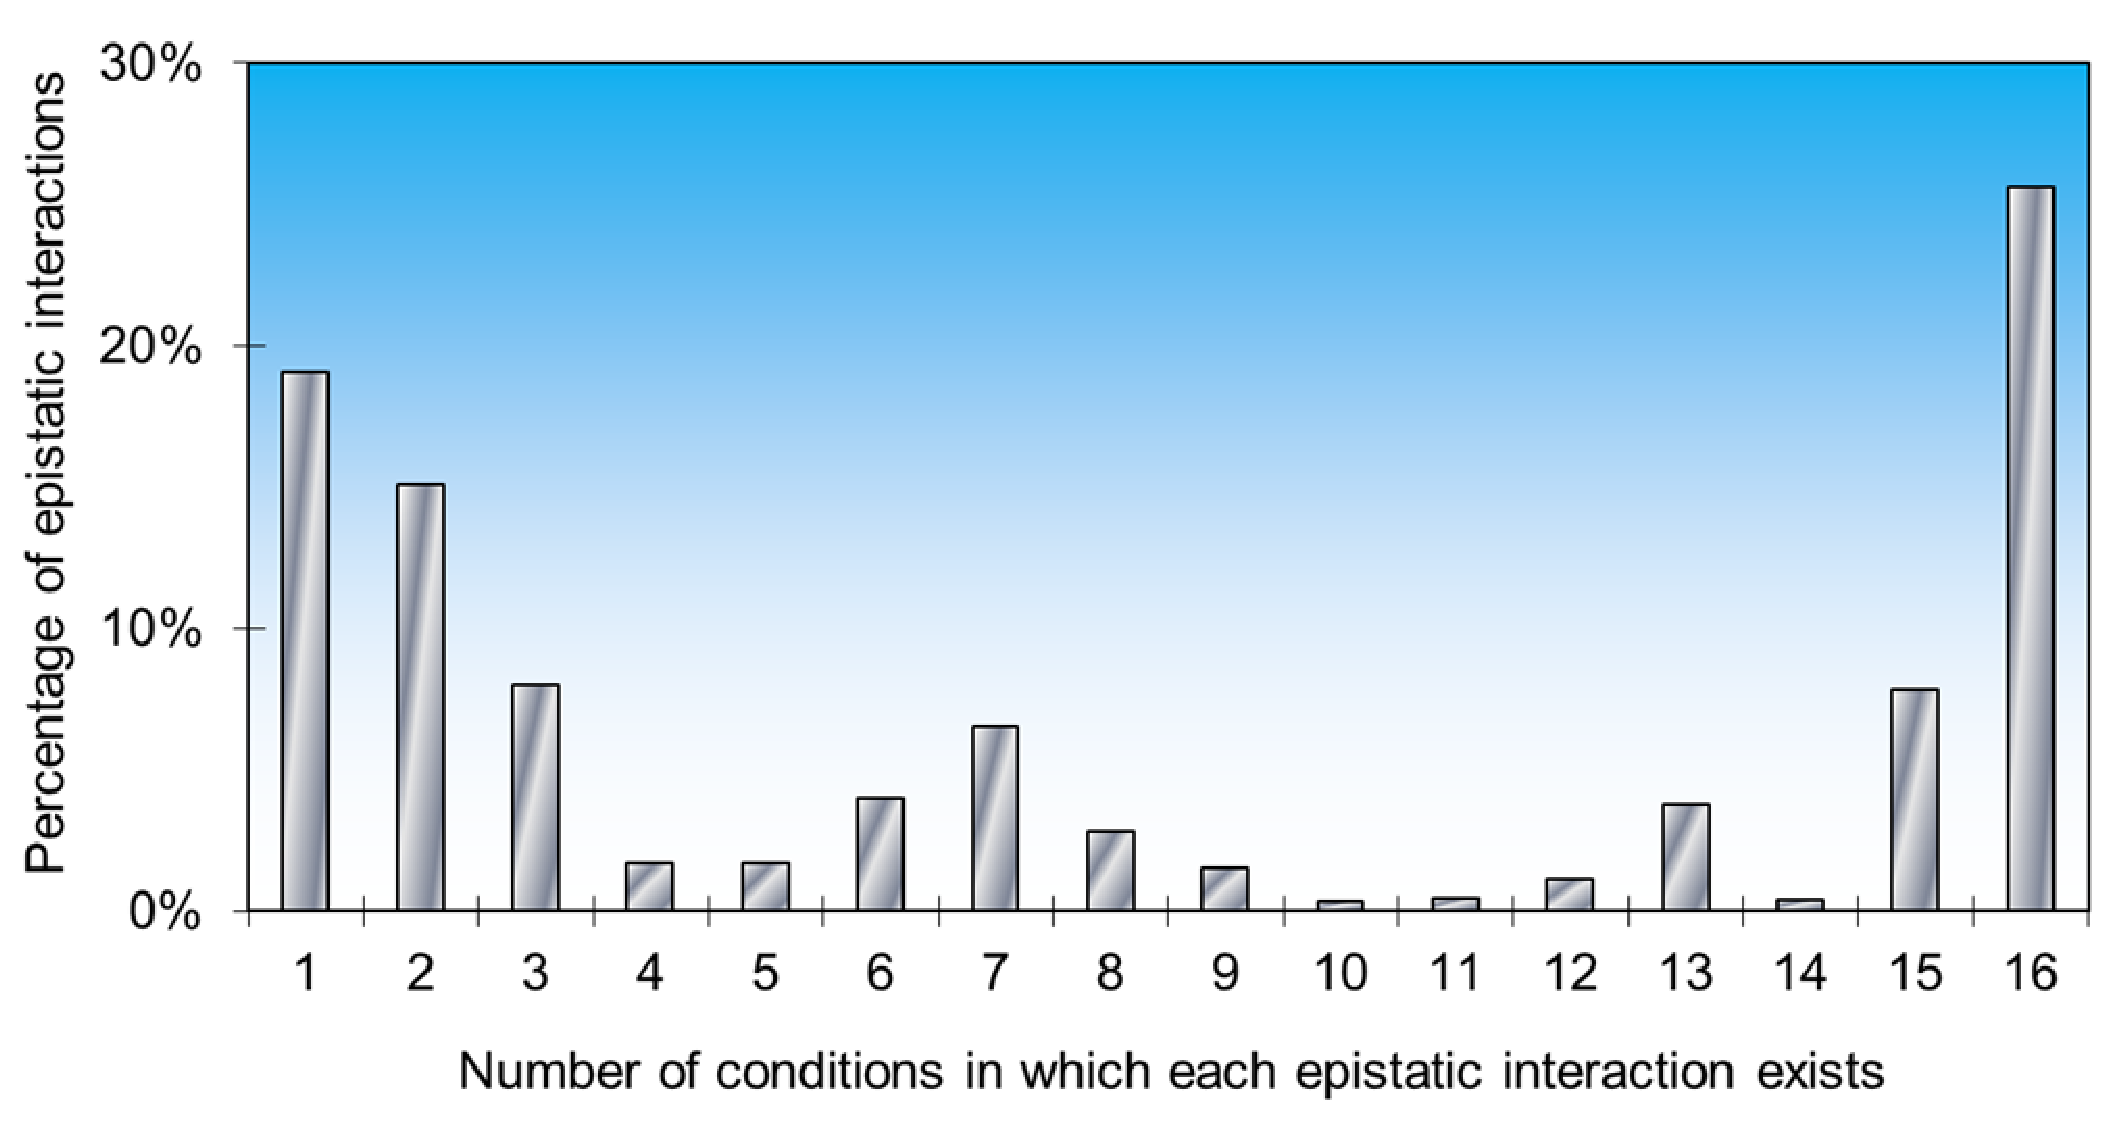
\includegraphics[width=\textwidth]{envFigure_S4}
\end{figure}

\end{document}